\section{Problem: Tiefensuche}

\begin{enumerate}
	\item[a.] Geben Sie Pseudocode für einen Algorithmus, der das folgende Problem löst: Gegeben ein zusammenhängender ungerichteter Graphen G, finde eine Weg, der jede Kante in G genau einmal in jeder Richtung durchläuft.\\
	\textit{Hinweis: Verwenden Sie Tiefensuche.}
	
	\item[b.] Sei G = (V, E) ein Graph. Gegeben ein Algorithmus, der in $O(|V |)$ Zeit überprüft, ob G genau einen Kreis enthält.\\
	\textit{Hinweis: Der Graph G muss nicht zusammenhängend sein. Wie müssen die
	Komponenten von G aussehen, wenn G genau einen Kreis enthält? Was haben Sie in Diskrete Strukturen über Bäume gelernt?}
\end{enumerate}

\subsection{Teilaufgabe a.}

\subsubsection{Pseudocode:} (In einem ungerichteten zusammenhängenden Graph findet der normaler DFS alle Knoten und durchläuft jede Kante zwei-mal (hin und zurück))

\begin{enumerate}
	\item initialisiere ein leeres Set visited (speichert ob ein Knoten bereichts besucht wurde) und ein Dictionary edge\_visits{} welches speichert wie oft eine Kante benutzt wurde.
	\begin{enumerate}
		\item initialisiere die Anzahl von Traversierungen / Durchläufe aller Kanten zunächst als 0 
	\end{enumerate}
	
	\item führe DFS mit dem Startknoten durch.
	\begin{enumerate}
		\item Ist der Aktuelle Knoten bereits besucht worden inkrementiere den Eintrag edge\_visit[aktuller\_Knoten][Vorgänger] um 1. (Backtracking gehe den Pfad den genommen wurde wieder zurück). Da der erste Knoten keinen Vorgänger hat kann von diesem auch nicht weiter gebacktracked werden. 
		\item wenn der aktuelle Knoten noch nicht besucht wurde füge ihn in das Set visited() ein.
		\item Inkrementiere den Dictionary Eintrag edge\_visits[aktueller\_Knoten][Nachbar] um 1.
		\item für jeden Nachbarn vom aktuellen Knoten führe den DFS aus. 
	\end{enumerate}
	
	\item in einem ungerichteten Knoten gilt: ${v,u} == {u,v}$, für $v,u$ in $V$ und ${v,u},{u,v}$ in $E$
	\item Jetzt sollten alle Kanten 2-mal traversiert worden sein, mittels der Tiefensuche.
\end{enumerate}

Jede Kante wurde 2-mal verwendet einmal hin und einmal zurück. das rückwärts traversieren passiert im normalen DFS normalerweise indirekt. Durch: besuche Nachbar$\rightarrow$Nachbar wurde bereits besucht$\rightarrow$starte keine weiter tiefensuche$\rightarrow$gehe den Weg wieder zurück.

Beispiel:
\usetikzlibrary{arrows.meta, positioning}
\begin{tikzpicture}[
	->,                        % alle Kanten mit Pfeil
	node distance=2cm and 2cm,
	every node/.style={circle, draw, minimum size=8mm, inner sep=0pt}
	]
	
	% Knoten
	\node (A) {A};
	\node (B) [right=of A] {B};
	\node (C) [right=of B] {C};
	\node (D) [right=of C] {D};
	
	\node (E) [below=of B] {E};
	\node (F) [below=of C] {F};
	
	% Kanten
	\draw (A) -- (B);
	\draw (B) -- (C);
	\draw (C) -- (D);
	\draw (B) -- (E);
	\draw (C) -- (F);
	\draw (E) -- (F);
	
\end{tikzpicture}


In einem ungerichteten Graphen gilt: $\{v,u\} = \{u,v\}$ für $v, u \in V$ und $\{v,u\}, \{u,v\} \in E$.

\vspace{1em}
\noindent\textbf{DFS Start bei Knoten 1:}

\begin{itemize}
	\item visited: $\{A\}$  
	edges\_num\_visits: $\{\text{A--B}: 0, \text{B--C}: 0, \text{C--D}: 0, \text{B--E}: 0, \text{E--F}: 0, \text{C--F}: 0\}$
	
	\item A--B besucht: visited: $\{A, B\}$  
	edges\_num\_visits: $\{\text{A--B}: 1, \text{B--C}: 0, \text{C--D}: 0, \text{B--E}: 0, \text{E--F}: 0, \text{C--F}: 0\}$
	
	\item A--B--C besucht: visited: $\{A, B, C\}$  
	edges\_num\_visits: $\{\text{A--B}: 1, \text{B--C}: 1, \text{C--D}: 0, \text{B--E}: 0, \text{E--F}: 0, \text{C--F}: 0\}$
	
	\item A--B--C--D besucht: visited: $\{A, B, C, D\}$  
	edges\_num\_visits: $\{\text{A--B}: 1, \text{B--C}: 1, \text{C--D}: 1, \text{B--E}: 0, \text{E--F}: 0, \text{C--F}: 0\}$
	
	\item zurück zu C: visited: $\{A, B, C, D\}$  
	edges\_num\_visits: $\{\text{A--B}: 1, \text{B--C}: 1, \text{C--D}: 2, \text{B--E}: 0, \text{E--F}: 0, \text{C--F}: 0\}$
	
	\item zu F: visited: $\{A, B, C, D, F\}$  
	edges\_num\_visits: $\{\text{A--B}: 1, \text{B--C}: 1, \text{C--D}: 2, \text{B--E}: 0, \text{E--F}: 0, \text{C--F}: 1\}$
	
	\item zu E: visited: $\{A, B, C, D, F, E\}$  
	edges\_num\_visits: $\{\text{A--B}: 1, \text{B--C}: 1, \text{C--D}: 2, \text{B--E}: 0, \text{E--F}: 1, \text{C--F}: 1\}$
	
	\item zurück zu B: visited: $\{A, B, C, D, F, E\}$  
	edges\_num\_visits: $\{\text{A--B}: 1, \text{B--C}: 1, \text{C--D}: 2, \text{B--E}: 1, \text{E--F}: 1, \text{C--F}: 1\}$
	
	\item zurück zu E: visited: $\{A, B, C, D, F, E\}$  
	edges\_num\_visits: $\{\text{A--B}: 1, \text{B--C}: 1, \text{C--D}: 2, \text{B--E}: 2, \text{E--F}: 1, \text{C--F}: 1\}$
	
	\item zurück zu F: visited: $\{A, B, C, D, F, E\}$  
	edges\_num\_visits: $\{\text{A--B}: 1, \text{B--C}: 1, \text{C--D}: 2, \text{B--E}: 2, \text{E--F}: 2, \text{C--F}: 1\}$
	
	\item zurück zu C: visited: $\{A, B, C, D, F, E\}$  
	edges\_num\_visits: $\{\text{A--B}: 1, \text{B--C}: 1, \text{C--D}: 2, \text{B--E}: 2, \text{E--F}: 2, \text{C--F}: 2\}$
	
	\item zurück zu B: visited: $\{A, B, C, D, F, E\}$  
	edges\_num\_visits: $\{\text{A--B}: 1, \text{B--C}: 2, \text{C--D}: 2, \text{B--E}: 2, \text{E--F}: 2, \text{C--F}: 2\}$
	
	\item zurück zu A: visited: $\{A, B, C, D, F, E\}$  
	edges\_num\_visits: $\{\text{A--B}: 2, \text{B--C}: 2, \text{C--D}: 2, \text{B--E}: 2, \text{E--F}: 2, \text{C--F}: 2\}$
\end{itemize}

\subsection{Teilaufgabe b.}
\subsubsection{Gesucht:}

Wie sehen die Komponenten des Graphen aus, damit genau ein Kreis im gesamten Graphen enthalten ist.

\subsubsection{Lösung/Ansatz:}

\paragraph{Kreis:} Was genau ist ein Kreis in einem Graph?\\
Ein Kreis in einem Graphen ist ein geschlossenen Pfad zwischen Start und Ziel, dabei gibt es keine Wiederholung von Knoten außer Start und Ziel.\\
Da wir nach \textbf{"genau ein Kreis"} suchen sollen, bedeutet das:
\begin{itemize}
	\item es darf \textbf{keinen} weiteren Kreis im Graphen geben
	\item und es \textbf{muss aber genau ein} Kreis vorhanden sein
\end{itemize}

\paragraph{Der Graph G muss nicht zusammenhänged sein:} Das bedeutet der Graph kann aus mehreren Teilkomponenten bestehen, also z.B.: aus zwei einzelne Graphen, die nebeneinander stehen, ohne Verbindung zueinander. D.h. der Kreis kann/darf (für diese Aufgabe) nur innerhalb einer der Zusammenhängenden Komponente entstehen, da ein Kreis ja ein geschlossener Pfad ist, müssen alle beteiligten Knoten und Kanten Verbunden sein.\\
Da es nicht mehr als ein Kreis geben darf, wären das andere Teilkomponent also Kreisfrei und damit also Baume.

\begin{center}
	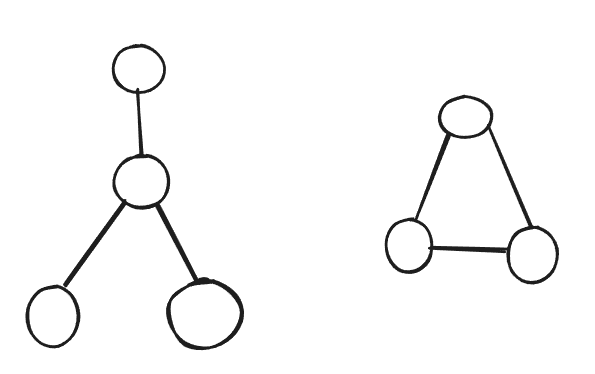
\includegraphics[scale=0.3]{Graph_Kreis}
\end{center}
\paragraph{Die Struktur von G bei genau einem Kreis:}
\begin{itemize}
	\item Der Graph $G$ besteht aus mehreren Teilkomponenten
	\item Nur einer dieser Teilkomponenten ist ein Baum mit zusätzlichen Kanten, die genau einen Kreis bilden
	\item Alle anderen Komponenten sind Bäume und Kreisfrei
\end{itemize}

\paragraph{Bäume aus Diskrete Strukturen:} 
\begin{enumerate}
	\item Ein Baum ist ein zusammenhängender, kreisfreier Graph
	\item In einem Baum gilt immer: $|E| = |V| - 1 $
	\item Wenn ein Kreis existiert, dann ist der Graph kein Baum mehr
\end{enumerate}